\section{Wstęp}
\begin{frame}{Wstęp}
	\textcolor{blue}{Sformułowanie zadania}$\newline$
	$\newline$
	\textbf{Dane:} $\newline$
 $m$ równań o m niewiadomych:
\begin{center}
$f_{i}(x_{1},\ x_{2},...,\ x_{j},...,\ x_{m})=0$; $i=1$, 2, $m... (*)$
$\newline$
\end{center}
\textbf{Warunek:}
$$
\vec{f}(\vec{x})=0
$$

\textbf{Rozwiązanie układu:}$\newline$ liczby $\alpha_{j}, j=1$, 2,..., $m$ takie że:
\begin{center}
$f_{i}(\alpha_{1},\ \alpha_{2},\ \alpha_{m})=0$;\  $i,\  j=1$, 2,..., $m$
\end{center}
\textbf{Uwaga:}$\newline$
Nie ma dobrych, ogólnych metod rozwiązania(*)
np. $m=2$
\end{frame}
\begin{frame}{Wstęp}
\begin{figure}[h]
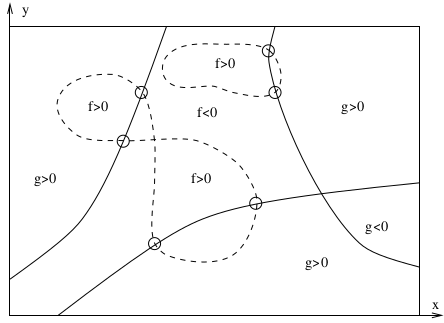
\includegraphics[width=0.75\linewidth]{img/9/9_1.png}
\end{figure}
$$
\left.\begin{array}{l}
f(x,\ y)=0\\
g(x,\ y)=0
\end{array}\right\} 
$$
 \end{frame}
\begin{frame}{Wstęp}
\textbf{Problemy:}
\begin{itemize}
\item kontury zerowe $\rightarrow$ podział płaszczyzny,
\item $\mathrm{f},\mathrm{g}-$dowolne $\Rightarrow$kontury bardzo złożone,
\item {\it liczba zer nie jest znana a priori},
\item dla $ x>2\rightarrow$hiperpłaszczyzny,
\item jak wybrać punkty startowe?
\item kiedy zakończyć poszukiwanie miejsc zerowych?
\item konieczność wyboru rozwiązania, którego poszukujemy $\rightarrow$ nie szukamy wszystkich
\end{itemize}

\textbf{Uwaga:}$\newline$
Wykorzystujemy wiedzę z analizy matematycznej, geometrii, algebry !!!
\end{frame}

\begin{frame}{Wstęp}
\textbf{Przykładowe układy równań nieiniowych - wizualizacja:}
$\newline$
\url{https://www.symbolab.com/solver/non-linear-system-of-equations-calculator}
$\newline$ $\newline$ 
\textbf{Zastosowanie układów równań nieliniowych:}
\begin{itemize}
	\item kinetyka reakcji chemicznych, badanie równowagi termodynamicznej układu, przewidywanie istnienia związków chemicznych
	\item sterowanie elektrycznymi silnikami prądu stałego
	\item badanie dynamiki samolotów (nieliniowe zależności prędkości, kątów,wysokości...)
	\item układy automatyczne, problem utrzymania równowagi w układach niestabilnych - drony
	\item ...
\end{itemize}
\end{frame}